\documentclass{beamer}

\usepackage{xcolor}
\usepackage{color}

\usepackage{graphicx}
\def\xcolorversion{2.00}
\def\xkeyvalversion{1.8}
\setbeamersize{text margin left=0pt,text margin right=0pt} 

\makeatletter
\newcommand*\bigcdot{\mathpalette\bigcdot@{.9}}
\newcommand*\bigcdot@[2]{\mathbin{\vcenter{\hbox{\scalebox{#2}{$\m@th#1\bullet$}}}}}
\makeatother


\usepackage{TIKZ_Macra}
\usepackage{xparse}


\usepackage[utf8]{inputenc}

\useinnertheme[shadow=true]{rounded}

\setbeamercolor{block title}{use=structure,fg=structure.fg,bg=structure.fg!30!bg}
%\setbeamercolor{block title}{fg=red}

\setbeamercolor{block body}{parent=normal text,use=block title,bg=block title.bg!50!bg}

\setbeamercolor{block title example}{use=example text,fg=example text.fg,bg=example text.fg!30!bg}
\setbeamercolor{block body example}{parent=normal text,use=block title example,bg=block title example.bg!50!bg}

%\usepackage{transparent}
\usepackage[most]{tcolorbox}
\usepackage{lmodern}
\usepackage{mathtools}
\usepackage{amsfonts}
\usepackage{amssymb}
\usepackage{latexsym}
\usepackage{hyperref}


\newtcbox{\mybox}{blank, on line, opacitytext=0.5}
\usepackage{changepage}

\usepackage{Moje_makra}

\usepackage{Moje_Zmienne}

\usepackage{Zbiory_i_konfiguracje}

\usepackage{Complexity}

\usepackage{Sieci}


\begin{document}

 


\begin{frame}{An Buchy automaton}
\Margines{
$\Sigma= \{a,b\}.$
  \begin{enumerate}
    \item<2-> Infinite number of $a$.
    \item<3-> Finite number of $a$
    \item<4-> Number of $b$ is infinite and number of $a$ between every two $b$ is divisible by $3.$
    \item<5-> Number of $a$ between every two $b$ is divisible by $3.$
    \item<6-> Number of $b$ is infinite and only finitely many times the number of $a$ between every two consecutive $b$ is divisible by $3.$
    \item<7-> Number of $b$ is finite and number of $a$ between every two consecutive $b$ is divisible by $3.$
    \item<8-> Number of $b$ is finite and number of $a$ between any two $b$ is not divisible by $3$.
   \end{enumerate}
}
\end{frame}


\begin{frame}{\Buchi\ languages}
\Margines{
\begin{lemma}
 For a given Kripke structure $S$ there is a \Buchi\ automaton $A$ such that:
 $$\lang{A}=\trace{S}.$$
\end{lemma}

\visible<2->{
\begin{block}{Lemma}
 Sets of languages accepted by \Buchi\ automata and generalised \Buchi\ automata are the same.
\end{block}}

\visible<3->{\begin{block}{Lemma}
 \Buchi\ languages are closed under:
 \begin{enumerate}
  \item Union,
  \item Intersection.
  \item Complement. (We will not do this)
  \item Determinisation does not work. (We need to extend the model)
 \end{enumerate}
\end{block}}
}
\end{frame}








\begin{frame}{LTL}
\Margines{
\begin{block}{}
Automata are not very convenient to write, it would be better to have some query language (logic).
\end{block}

\begin{block}{Definition}
 An $LTL$ formula $\phi$ is generated according a following rules:
 $$\phi \rightarrow true | p_i\in \AProp | \phi_1\land \phi_2 | \neg \phi_1 | X \phi_{1} | \phi_1 U \phi_2 $$
\end{block}
}
\end{frame}


\begin{frame}{Semantics of LTL}
\Margines{
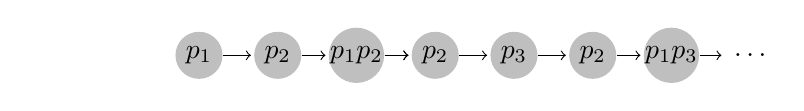
\begin{tikzpicture}[shorten >=1pt,->]
  \tikzstyle{vertex}=[circle,fill=black!25,minimum size=17pt,inner sep=0pt]

  \node[] (zero) at (-1,0) {$\ $};
  \foreach \name/\p/\x in {1/p_1 /1, 2/p_2/2, 3/p_1 p_2/3, 4/p_2/4, 5/p_3/5, 6/p_2/6, 7/p_1 p_3/7}
    \node[vertex] (G-\name) at (\x,0) {$\p$};

    \node[] (G-kropki) at (8,0) {$\ldots$};

  \foreach \from/\to in {1/2,2/3,3/4,3/4,4/5, 5/6, 6/7, 7/kropki}
    \draw (G-\from) -> (G-\to);
\end{tikzpicture}

\begin{itemize}
 \item $true \iff true$.
 \item $p_1 \iff p_1\text{ holds at position 0}.$
 \item $p_2 \iff p_2\text{ holds at position 0}.$
 \item $p_1 \land p_2 \iff p_1\text{ and }p_2\text{ holds at position 0} .$
 \item $\neg p_2$ $\iff p_2\text{ does not hold at position 0} .$
 \item $X p_2 \iff p_2\text{ holds at position 1} .$
 \item $XX (p_1\land p_2) \iff p_2\text{ and } p_1\text{ holds at position 2}.$
 \item $\neg (\neg p_1 \land \neg p_2) U p_3$ $\iff \text{ there is } 0\leq j \text{ such that }
 p_3\text{ holds at position j and }\neg (\neg p_1 \land \neg p_2) \text{ holds for all } 0\leq i<j.$
\end{itemize}

}
\end{frame}

\begin{frame}{Exercise}
\Margines{
 How to express:
 \begin{enumerate}
 \item Finally there will be a state in which $p_2$ holds.\par
 \visible<2->{$F p_2$}
 \item<3-> Every state along the path satisfy $p_2$.\par
 \visible<4->{$G p_2$}
 \item<5-> If $p_2$ holds at the state with index $2$ then $p_3 \lor p_1$ holds in the state with index $4$.

 \item<6-> If in some state $p_1$ is satisfied then in the future $p_2$ has to be satisfied.
 \end{enumerate}

}
\end{frame}


\begin{frame}{How to verify LTL formula?}
\Margines{
\begin{block}{Lemma}
Let $\words{\phi}$ denotes a set of words that satisfy the LTL formula $\phi$.
For a given LTL formula $\phi$ one can construct an exponential size \Buchi\ automaton $B$ recognising exactly the same set of words, i.e.
$$\lang{B}= \words{\phi}$$
\end{block}
\begin{enumerate}
 \item Build an automaton $A$ for the Kripke structure.
 \item Build an automaton $B$ for $\phi$ an LTL formula,\par
 or build an automaton $B$ for $\neg \phi$.
 \item Check nonemptiness of $\lang{A}\cap\lang{B}.$
 \end{enumerate}

}
\end{frame}


\begin{frame}{How to verify LTL formula?}
\Margines{
\begin{block}{Lemma}
Let $\words{\phi}$ denotes a set of words that satisfy the LTL formula $\phi$.
For a given LTL formula $\phi$ one can construct an exponential size \Buchi\ automaton $B$ recognising exactly the same set of words, i.e.
$$\lang{B}= \words{\phi}$$
\end{block}

}
\end{frame}


\begin{frame}{Bibliography}
 \Margines{
 Units from 3 to 8 from

	\url{https://www.youtube.com/channel/UCUXDMaaobCO1He1HBiFZnPQ/videos}%{https://www.youtube.com/channel/UCUXDMaaobCO1He1HBiFZnPQ}

There are a lot of videos first one is "A problem in concurrency".

 }
\end{frame}



\end{document}
